% SLOGAN: This chapter formally introduces "the maintenance view."
% Sticky sentence: "Categories are real because they are maintained."
% See notes/book-slogans.md for the book-wide slogan strategy.

\chapter{Kinds without essences}
\label{ch:kinds-without-essences}

\epigraph{You should consider that the essential art of civilization is maintenance.}{Pete Seeger, quoted in \citet{brand2024}}

Part I raised a question: if categories aren't defined by essences, what makes them real? The answer this chapter develops is simple: categories are real because they are maintained. This is the \term{maintenance view}.

The word \enquote{maintenance} is chosen deliberately. Stewart Brand's recent work on infrastructure, buildings, and software makes a point that applies equally to grammar: maintenance isn't just preventing breakdown; it's the whole process of keeping something going \citep{brand2024}. Monitoring, repair, renewal, adaptation~-- these are what keep bridges standing and cities functioning. Brand's insight is that we systematically undervalue maintenance because its successes are invisible: a well-maintained system just \emph{works}, and we notice only when it fails.

Grammatical categories are like this. When they function smoothly~-- when speakers agree on what counts as a noun, when learners acquire the same categories their parents have~-- the maintenance is invisible. We notice the mechanisms only at the boundaries, where the system creaks: the words that won't classify, the constructions that shift between generations, the gradience that essentialism can't explain. Brand's framing helps: think of the mechanisms not as defining the categories but as maintaining them. The categories are real because the maintenance is continuous.

The idea of maintenance as constitutive~-- not just preservative~-- comes from philosophy of biology. Species aren't defined by genetic essences~-- no checklist of necessary and sufficient conditions separates one species from another. But species are real. They support induction, figure in explanations, persist across time. What makes them real is not a shared essence but a shared causal history: mechanisms of reproduction, selection, and development that keep certain properties clustering together.

Richard Boyd called these \term{homeostatic property cluster kinds}~-- or HPC kinds \citep{boyd1991,boyd1999}. The name is technical but its parts are revealing. \emph{Stasis}: standing, position~-- the cluster \emph{stays} in place, maintained by ongoing processes. \emph{Homeo}: same, similar~-- when disturbed, the cluster tends to return to the \emph{same} configuration, not just any stable state. A homeostatic system doesn't merely persist; it self-corrects. Perturb a species' genome and selection pushes back toward the original distribution. Isolate a population and reproductive barriers emerge that restore the clustering. The name captures both the \emph{staying} and the \emph{sameness}~-- stability is not just inertia but active return.

Think of a spinning top. It stays upright not because it's rigid but because it's moving. The spin resists perturbation~-- push it slightly and gyroscopic forces bring it back. Stop the spin and the top falls. Homeostatic kinds are like this: their stability is dynamic, not static. What keeps the cluster clustered is not a fixed structure but an ongoing process.

\begin{figure}[t]
\centering
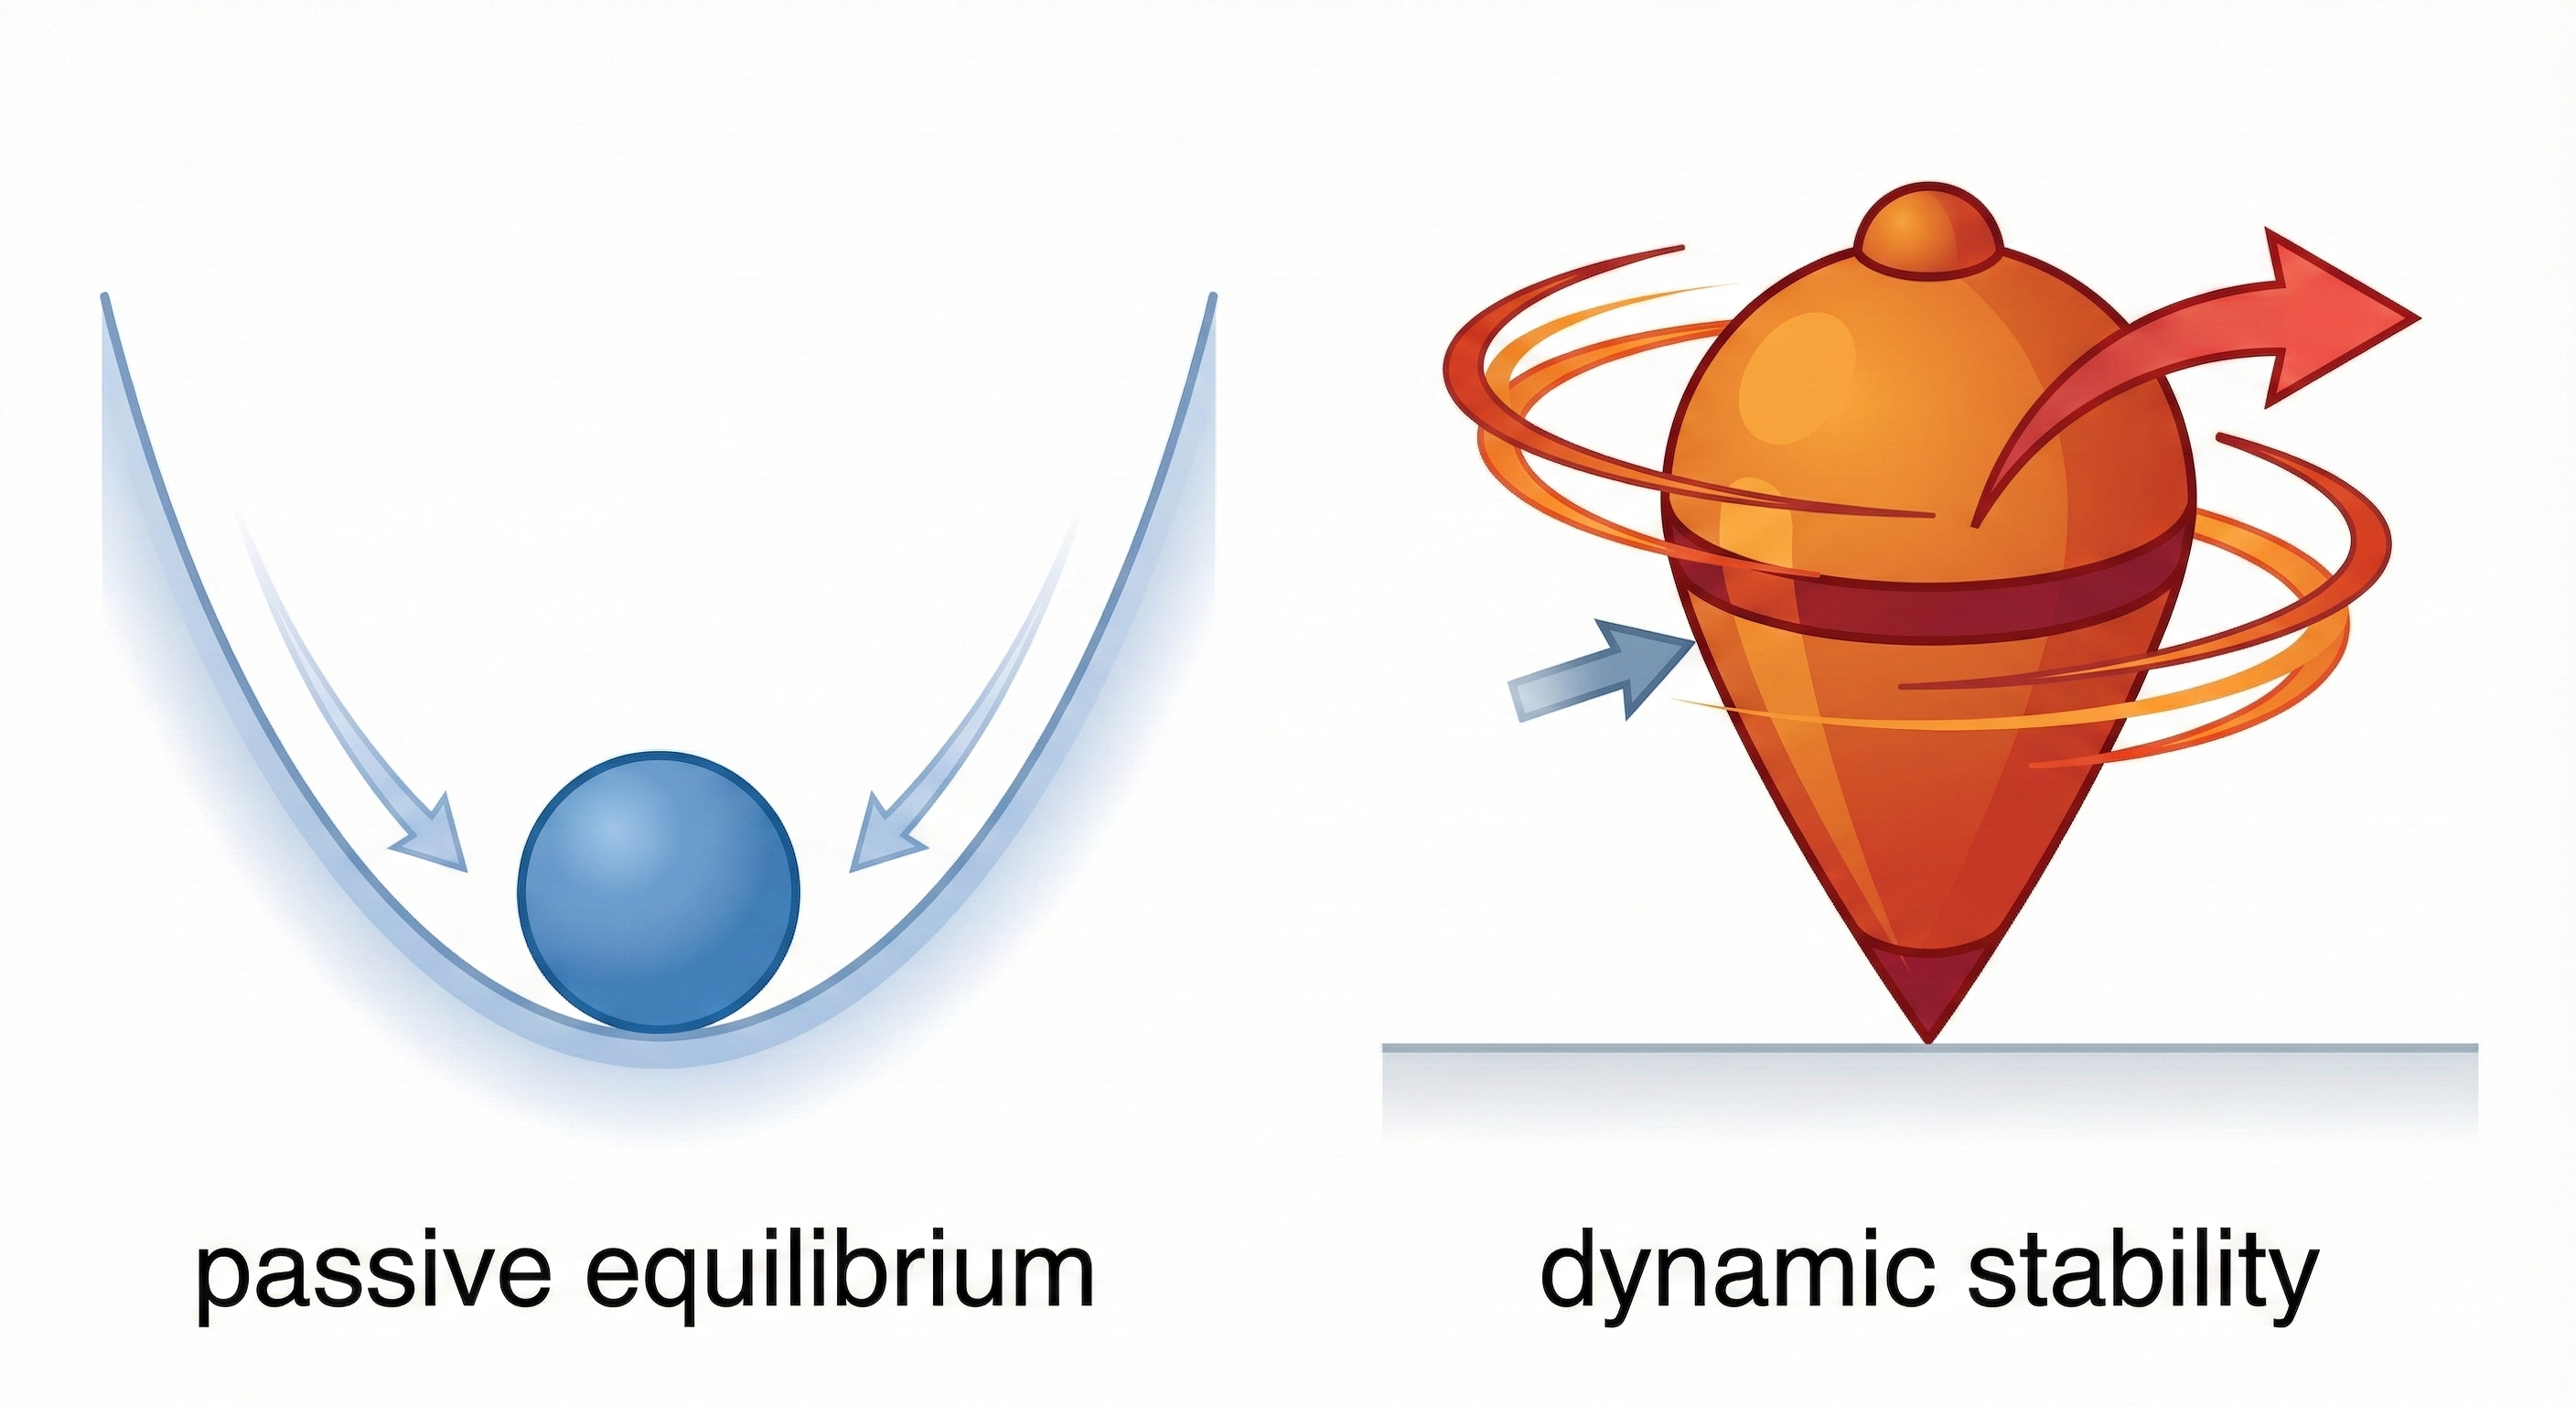
\includegraphics[width=0.75\textwidth]{figures/4.top-vs-ball.png}
\caption{Two kinds of stability. Left: a ball at the bottom of a valley is in passive equilibrium~-- it settles where gravity deposits it. Right: a spinning top maintains dynamic stability~-- the spin actively resists perturbation, and when pushed, gyroscopic forces push back. Homeostatic property cluster kinds are like the top: their stability is achieved through ongoing processes, not through static structure.}
\label{fig:top-vs-ball}
\end{figure}

And the maintenance needn't be entirely external. Some of the stability arises from reciprocal reinforcement among the clustered properties themselves. Recall \textit{Smilodon} and \textit{Thylacosmilus} from Chapter~\ref{ch:essentialism} (Figure~\ref{fig:convergent-morphology}): their massive canines, powerful forelimbs, solitary hunting, and apex-predator niche aren't accidentally co-present. They are causally interlocking~-- each makes the others more likely, more stable, more resistant to drift. Large canines require the musculature to wield them; ambush predation requires the solitude to stalk; apex status requires the whole package. The cluster is a self-stabilising network, embedded in broader developmental, ecological, and transmission dynamics. This is the reflexive dimension of homeostasis: the properties, by virtue of being those properties, participate in maintaining the cluster.


\section{From species to categories}
\label{sec:4:species-to-categories}

The biological parallel isn't decorative. Species and grammatical categories face the same philosophical problem: both look like natural kinds~-- they support induction, figure in explanations, persist across time~-- but neither has an essence in the classical sense. No genetic sequence is necessary and sufficient for tigerdom; no morphosyntactic property is necessary and sufficient for nounhood. But tigers are real, and so are nouns. The question is how.

Boyd's answer for species was that the clustering does the epistemic work while the mechanisms explain the clustering. Tigers share properties~-- striped fur, carnivorous diet, solitary hunting, particular vocalisations~-- not because these properties define \term{tiger} but because the mechanisms of reproduction, development, and selection keep them bundled together. The properties vary; not every tiger has all of them. But they cluster reliably enough that learning about one tiger tells you something about others. That's what makes \term{tiger} projectible~-- able to support inductive inference~-- even without a definition.

The same logic applies to grammatical categories. Nouns share properties~-- they head noun phrases, occur with determinatives, inflect for number, denote entities~-- not because these properties define \term{noun} but because the mechanisms of acquisition, entrenchment, and transmission keep them bundled. The properties vary; not every noun has all of them. But they cluster reliably enough that learning the category \term{noun} tells you something about how unfamiliar nouns will behave.

Ruth Millikan's work on \term{copied kinds} sharpens the parallel \citep{millikan1984,millikan2017}. A copied kind is a category whose members are produced from each other or from a common template~-- they share properties because they share a lineage, not because they share an essence. Biological species are copied kinds: each organism is a copy (with variation) of its parents. Artefacts like screwdrivers are copied kinds: each is produced from a template (with variation) that was itself copied from earlier templates.

Grammatical categories are copied kinds par excellence. Each generation doesn't invent nouns from scratch; children copy the category from their input, with variation, and pass it on. The properties cluster because the copying is high-fidelity enough to preserve them. The variation accumulates because no copying is perfect. The category persists because the lineage persists~-- an unbroken chain of transmission from speaker to speaker across millennia. Khalidi calls such history-defined kinds \term{etiological kinds} and defends their status as genuine natural kinds \citep[106--112]{khalidi2013}.

This is what makes the biological parallel load-bearing rather than merely illustrative. The mechanisms maintaining species cohesion~-- reproduction, gene flow, selection, developmental constraint~-- have genuine analogues in language. Not identical mechanisms, but mechanisms playing the same structural role: keeping properties clustered, filtering variation, stabilising the kind across time.

\begin{table}[t]
\centering
\caption{Parallel mechanisms in biology and grammar}
\label{tab:parallel-mechanisms}
\begin{tabular}{@{}lll@{}}
\toprule
\textbf{Function} & \textbf{Biological mechanism} & \textbf{Linguistic mechanism} \\
\midrule
Transmission & Reproduction & Acquisition \\
Filtering & Natural selection & Communicative success \\
Cohesion & Gene flow & Interactive alignment \\
Constraint & Development & Processing limitations \\
Attraction & Ecological niche & Functional pressure \\
\bottomrule
\end{tabular}
\end{table}

Table~\ref{tab:parallel-mechanisms} sketches the correspondences.\footnote{These are functional analogues, not homologues: the mechanisms occupy the same position in an explanatory structure without sharing causal architecture. Analogy is scientifically respectable; the parallel is load-bearing but not a claim of identity.} Not every detail maps, and that's fine. The claim isn't that language \emph{is} biology but that the same style of explanation works: mechanism-based, historical, non-essentialist. What maintains the clustering matters more than what defines the category.


\section{What mechanisms mean}
\label{sec:4:mechanisms}

\term{Mechanism} is doing a lot of work in this account, so I should say what I mean by it. I don't mean anything fancy~-- not the elaborate machinery of mechanistic philosophy of science, though that literature is relevant \citep{machamer2000,craver2007}. I mean something simpler: a process that reliably produces an outcome.

A mechanism, in this sense, has inputs, operations, and outputs. The inputs are whatever the process operates on~-- for acquisition, the input is linguistic data; for entrenchment, the input is frequency of use. The operations are what the process does~-- extracting patterns, strengthening associations, coordinating with interlocutors. The outputs are the effects~-- categories learned, habits formed, norms aligned.

The mechanisms maintaining grammatical categories aren't mysterious. They're the processes that usage-based linguistics has been studying for decades: statistical learning, exemplar storage, analogical extension, routinisation. What HPC adds is a way of understanding what these mechanisms collectively accomplish. They don't just shape individual grammars; they maintain categories as real kinds~-- clusters of properties that persist across speakers and generations.

One clarification. When I say mechanisms \enquote{maintain} categories, I don't mean they keep categories frozen. Maintenance includes change. A well-maintained building gets renovated; a well-maintained codebase gets refactored. The point of maintenance is that the system keeps functioning, not that it stays identical. Grammatical categories change~-- \mention{fun} drifts toward adjectives, \mention{will} grammaticalises from lexical verb to auxiliary~-- and these changes are themselves produced by the mechanisms. The category persists because the mechanisms keep operating, even as they reshape what the category contains.

This distinguishes HPC from both essentialism and prototype theory. Essentialism locates category identity in a definition~-- change the definition and you change the category. Prototype theory locates category identity in a central exemplar~-- but doesn't explain why the prototype stays central. HPC locates category identity in the mechanisms~-- the category is whatever the mechanisms maintain. Change the mechanisms and you change the category. Keep the mechanisms operating and the category persists, even as its boundaries shift.


\section{The mechanisms themselves}
\label{sec:4:the-mechanisms}

Let me name the mechanisms concretely. This isn't an exhaustive list~-- Chapter~\ref{ch:homeostasis} develops the full picture~-- but it's enough to show that \enquote{mechanisms maintain categories} isn't hand-waving.

\subsection{Acquisition}
\label{subsec:4:acquisition}

Children acquire grammatical categories without being taught definitions. No parent explains that nouns are words that can be preceded by determinatives and followed by plural suffixes. But children converge on the same categories their parents have, reliably, across cultures, in just a few years~-- which is more than most PhD students manage.

How? Not by innate specification~-- that just relocates the essence to the genome and doesn't explain why categories vary across languages. The HPC answer is that children track statistical regularities that reflect the underlying mechanisms. They acquire categories by being sensitive to the pressures that maintain them.

The evidence is strong. Distributional learning~-- tracking which words occur in which contexts~-- is sufficient to induce grammatical categories from raw input \citep{redington1998,mintz2003,piantadosi2024,kallini2024}. Infants are sensitive to these distributions from early in the first year \citep{gomez2000}. The categories children induce match adult categories not because children have innate category templates but because the same distributional patterns that define adult categories are present in child-directed speech.

Acquisition is a mechanism of maintenance because it transmits categories across generations. Each child who learns \term{noun} from input and then uses nouns in ways the next generation can learn from keeps the category alive. The mechanism is imperfect~-- children don't reproduce their parents' grammars exactly~-- and this imperfection is itself important. Variation enters through acquisition; selection operates on that variation; categories evolve. But evolution isn't dissolution. The category persists because acquisition is reliable enough, even though it isn't perfect.

\subsection{Entrenchment}
\label{subsec:4:entrenchment}

Frequency matters. High-frequency items are processed faster, stored more robustly, and resist analogical pressure more strongly than low-frequency items \citep{bybee2006,diessel2007}. This is \term{entrenchment}: the deepening of mental representations through repeated use.

Entrenchment maintains categories by anchoring them. The most frequent nouns~-- \mention{thing}, \mention{time}, \mention{way}, \mention{people}~-- are processed automatically, without conscious categorisation. They're the bedrock of the category, the items that every speaker agrees on, the prototypes around which less frequent items cluster. Change the behaviour of \mention{thing} and you change what \term{noun} means. Good luck. \mention{Thing} is so entrenched that changing it is nearly impossible~-- it would require shifting the habits of every English speaker simultaneously.

High-frequency items also grammaticalise faster. The path from lexical verb to auxiliary~-- \mention{will}, \mention{going to}, \mention{have to}~-- runs through frequent, semantically general items. Low-frequency items don't grammaticalise because they're not processed often enough to undergo the phonetic reduction and semantic bleaching that grammaticalisation requires. The category \term{auxiliary} exists because entrenchment creates a basin of attraction: items that enter the basin get pulled toward the prototype; items outside it stay lexical.

Entrenchment also determines which syntactically well-formed expressions count as grammatical in context. In English, the way to ask about someone's age is \mention{How old are you?}, with the response \mention{I'm forty} or \mention{I'm forty years old}. The calque from French would be \mention{What age do you have?} and \mention{I have forty years.} These clauses violate no syntactic rules of English, but the first set is entrenched and the second is not. As a result, the second set is not just unacceptable but ungrammatical as age-question pairs~-- though \mention{I have forty years} is perfectly fine as a response to a query about time until retirement. The grammaticality of an expression can depend on its entrenchment within a particular functional slot, not just its structural well-formedness.

\subsection{Interactive alignment}
\label{subsec:4:alignment}

Speakers accommodate to each other. In conversation, interlocutors converge on lexical choices, syntactic structures, even phonetic details \citep{pickering2004,garrod2009}. This is \term{interactive alignment}: the tendency to match your speech to your interlocutor's.

Alignment maintains categories by enforcing community-wide coherence. If I use \mention{adult} as a verb and you accommodate, we've both reinforced the verb use. If you resist~-- if you pointedly say \mention{be responsible} instead~-- you've exerted pressure against the innovation. Either way, the interaction shapes subsequent usage. Multiply this by millions of conversations and you get a distributed mechanism for maintaining shared norms.

The alignment needn't be conscious. Most accommodation is automatic, below the level of awareness. Speakers don't decide to match their interlocutors' syntax; they just do. This automaticity makes alignment a powerful stabilising force. Categories persist not because speakers explicitly agree on them but because speakers implicitly coordinate, conversation by conversation, year by year.

\subsection{Iterated transmission}
\label{subsec:4:transmission}

Language is transmitted imperfectly across generations. Children don't reproduce their parents' grammars exactly; each generation introduces variation. You might expect this imperfection to degrade structure~-- random errors accumulating until categories dissolve into noise. But the opposite happens. Structure emerges.

Simon Kirby and colleagues demonstrated this experimentally \citep{kirby2008,kirby2015compression}. Participants learned an artificial language~-- nonsense words paired with meanings~-- and then reproduced it for the next \enquote{generation.} The initial language was arbitrary: no pattern connected form to meaning. By generation ten, the language had become compositional~-- word parts systematically encoded meaning components. Structure emerged from the transmission process itself, as learnable variants outcompeted arbitrary ones.

The mechanism is a filter. Not all variants survive transmission equally. Easy-to-learn variants get reproduced faithfully; hard-to-learn variants get distorted or lost. Over generations, this filtering selects for systematicity. Languages become more learnable because learnable languages survive transmission; unlearnable ones don't.

For grammatical categories, the implication is direct. Categories that are easy to acquire~-- categories with clear distributional signatures, consistent morphological marking, coherent semantic cores~-- survive transmission better than categories without these properties. The categories we observe today are the residue of this filtering process, iterated across thousands of generations. They're structured because only structured categories could have survived.

\subsection{Functional pressure}
\label{subsec:4:functional}

Categories exist because they do something. Nouns package referents for tracking across discourse. Verbs encode events and their participants. Determinatives signal identifiability. The functions aren't arbitrary~-- they reflect communicative needs that languages address.

Functional pressure maintains categories by making them useful. A language without nouns would struggle to establish reference; a language without verbs would struggle to predicate. These aren't logical necessities~-- you can imagine communication systems without such categories~-- but they're practical near-necessities for the kinds of communication humans engage in: extended discourse, complex reference, hierarchical structure.

Where functional pressure is strong, categories are stable. Something like the noun--verb distinction emerges in nearly all documented languages~-- even where the surface realisations differ radically~-- because the functions nouns and verbs serve are so widely needed. Where functional pressure is weak, categories vary. Not all languages distinguish adjectives from nouns; not all languages have adverbs as a distinct category. The functions these categories serve can be performed by other means~-- nouns can modify nouns; verbs can modify verbs~-- so the pressure to maintain them as separate kinds is lower.

Functional pressure also shapes category boundaries. The core of a category~-- the items where clustering is tightest~-- consists of items that serve the function most directly. The periphery consists of items that serve the function less well or serve multiple functions. This is why prototypes are prototypes: they're not arbitrary central exemplars but the items that best perform the category's function.


\subsection{Homeostasis or simple causation?}
\label{subsec:4:homeostasis-causation}

A critic might grant that mechanisms matter but question whether \emph{homeostasis} is the right word. Muhammad Ali Khalidi, in a systematic critique of Boyd's HPC framework, argues that the homeostatic requirement is too restrictive \citep[72--79]{khalidi2013}. Many natural kinds~-- including paradigmatic ones like biological species~-- don't maintain equilibrium. Species evolve; the properties associated with them shift over generations. If homeostasis means returning to a stable state when perturbed, then evolving species don't qualify. Yet they're surely natural kinds.

Khalidi proposes a \term{simple causal theory} as an alternative: natural kinds are associated with properties where some (primary) cause others (secondary), without requiring feedback loops or self-correction. On this view, what matters is causal structure, not equilibrium. The kind \mention{polymer} exemplifies the pattern: the primary property (consisting of long chains of repeating monomers) causes the secondary properties (viscosity, rigidity, no gaseous phase), but there's no mechanism pushing polymers back toward some ideal state. The causation is one-way, from structure to behaviour.

The critique deserves a careful response, because grammatical categories might work differently from biological ones.

For some grammatical categories, Khalidi's simpler picture may be adequate. What I called \emph{thin} categories~-- nonce coinages, idiolectal forms, ephemeral patterns that never stabilise~-- might indeed be merely causal. They have properties that cluster because function causes structure: a word coined to package a referent takes on nominal properties. But there's no feedback, no correction, no return to equilibrium when perturbed. The category exists only as long as the functional pressure persists; perturb it and it drifts or dissolves.

But for robust categories~-- the ones that persist across speakers and generations, that resist innovation, that pull deviant items back toward the prototype~-- something stronger is operating. The mechanism of \emph{interactive alignment} is the key test case. When I use \mention{adult} as a verb and you accommodate, we've jointly reinforced the pattern. But when you resist~-- when you pointedly say \mention{be responsible} instead~-- you've exerted corrective pressure. The interaction didn't just transmit a pattern; it pushed back against deviation. That's homeostasis in the original sense: a system-level tendency to return to the same state, not just any stable state.

The spinning top metaphor from earlier captures the difference. Khalidi's simple causal theory describes a ball rolling downhill: structure causes behaviour, and the ball comes to rest wherever the slope deposits it. Homeostasis describes a spinning top: the spin actively resists perturbation, and when disturbed, the top returns to upright rather than settling into whatever orientation gravity provides. The question for each category is: ball or top? Passive drift or active return?

The answer will vary. Closed-class categories~-- determinatives, auxiliaries, subordinators~-- are heavily entrenched and tightly aligned. Speakers agree on what they are; innovations are rare and resisted. These behave like tops. Open-class categories~-- nouns, verbs, adjectives~-- are more variable at the margins. High-frequency items are top-like (try changing how \mention{thing} works); low-frequency items may be ball-like (nonce uses drift without correction). The HPC label applies best where feedback operates. Khalidi's simpler model may suffice for categories maintained by unidirectional causation.

This heterogeneity is expected. Khalidi is right that not all kinds are homeostatic; the maintenance view accommodates this by allowing that different mechanisms maintain different kinds. The question \enquote{is this category genuinely homeostatic?} becomes empirical rather than definitional. And the diagnostic is concrete: does the category exhibit corrective feedback (alignment resisting innovation, entrenchment anchoring prototypes, transmission filtering anomalies), or does it merely exhibit one-way causation (function producing structure, with no path back)?

For the grammatical categories this book focuses on~-- the major parts of speech, the core morphosyntactic features, the constructions that persist across generations~-- the evidence favours homeostasis. These are categories where speakers correct each other, where high-frequency items anchor low-frequency ones, where transmission filters out deviants. They're not static~-- the spinning top precesses, the categories evolve~-- but they're also not passively drifting. Something is keeping them upright.


\section{What you get in return}
\label{sec:4:payoffs}

We've been framing this negatively~-- kinds \emph{without} essences. The positive formulation matters more: kinds \emph{with} mechanisms, \emph{with} stability, \emph{with} explanatory power. From here on, the question is what maintains categories, not what they lack.

Abstract frameworks are worth adopting only if they pay their way. What does the maintenance view buy that essentialism and prototype theory don't?

First, \textbf{boundary cases become data}. On the essentialist view, words like \mention{fun} or \mention{near} that don't fit standard categories are embarrassments~-- evidence that the definitions need refining, or that the words are somehow defective. On the HPC view, these words are exactly what you'd expect. They're items near basin boundaries, where multiple mechanisms pull in different directions. Their instability isn't noise; it's evidence about where the boundaries lie and which mechanisms are operating. The framework transforms anomalies into informants.

Second, \textbf{variation becomes tractable}. Essentialism has trouble with the fact that speakers disagree about category membership~-- is \mention{fun} an adjective or not? If categories are defined, disagreement means someone is wrong. On the HPC view, variation is expected. Different speakers have different input histories, different entrenchment profiles, different interlocutors to align with. Their categories will differ at the margins even if they agree at the core. The framework predicts variation and tells you where to expect it: near boundaries, for low-frequency items, in rapidly changing constructions.

Third, \textbf{diachrony becomes visible}. Categories change~-- \mention{will} was a lexical verb; now it's an auxiliary. Essentialism treats change as replacement: the old category dies and a new one is born. But that's not what happens phenomenologically. \mention{Will} didn't stop being a verb and start being an auxiliary overnight; it drifted, gradually, across a fuzzy boundary. The HPC view makes this visible: the mechanisms shifted, the basin migrated, the item moved from one cluster to another. Diachrony is category maintenance observed over longer timescales.

Fourth, \textbf{cross-linguistic comparison becomes empirical}. The typologist's question~-- do all languages have adjectives?~-- looks different under HPC. It's not about whether languages have categories that match a definition; it's about whether the same mechanisms produce the same clustering cross-linguistically. If the mechanisms that maintain adjectives in English also operate in Mandarin, then Mandarin has adjectives in the relevant sense~-- even if the surface patterns differ. If different mechanisms are operating, then the comparison fails. The question becomes tractable because it's about mechanisms, not definitions. Chapter~\ref{ch:word-classes} develops this in detail.

Fifth, \textbf{the \enquote{right analysis} question transforms}. Linguists spend enormous effort debating whether some item is \enquote{really} a noun or \enquote{really} a verb, whether some construction is \enquote{really} a clause or \enquote{really} a phrase. Under essentialism, these questions have determinate answers: the item either satisfies the definition or it doesn't. Under HPC, the questions are reframed. The issue isn't which definition is correct but which mechanisms are operating. An item can be genuinely intermediate~-- subject to mechanisms that pull it toward multiple categories~-- without anyone being wrong about what it is.


\section{Sciences that made the shift}
\label{sec:4:precedents}

Linguistics isn't the first science to confront the limits of essentialism. The shift from definitional to mechanistic thinking has precedents, and they're reassuring: the sciences that made the shift became more productive, not less.

Biology is the paradigm case. Pre-Darwinian biology sought essences~-- the form of the horse, the essence of the mammal. Species were natural kinds with definitions, even if the definitions were elusive. Darwin dissolved this picture. Species became populations~-- statistical aggregates of varying individuals, maintained by mechanisms of reproduction and selection, without fixed boundaries or defining properties. The shift was wrenching. It felt like giving up on rigour, abandoning the very idea of natural kinds.

But biology flourished. Population thinking~-- Ernst Mayr's term for the anti-essentialist perspective~-- enabled modern evolutionary biology, ecology, and genetics \citep{mayr1959,mayr1982}. The same variation that embarrassed essentialism became the raw material for evolutionary theory. Species boundaries, once problematic because fuzzy, became informative because the fuzziness revealed ongoing evolutionary processes. The mechanisms of maintenance~-- selection, drift, gene flow~-- became the central objects of study.

Chemistry tells a different story but with the same moral. Pre-modern chemistry sought essences too~-- the essence of gold, the principles underlying material transformation. The essentialist picture collapsed, but what replaced it wasn't mechanism-talk; it was structural chemistry. Gold is the element with atomic number 79~-- not because 79 protons define goldness but because atomic number determines chemical behaviour. The \enquote{essence} was relocated from manifest properties to causal structure.

The move from \enquote{what properties define the kind} to \enquote{what structure explains the clustering} is the same move HPC makes for grammatical categories. The issue isn't finding the right definition of \term{noun}; it's identifying the causal-structural facts that make nouns cluster. The facts are distributed~-- they're in acquisition, entrenchment, alignment, transmission, function~-- but they're no less real for being distributed.

Psychology went through a similar transition in the prototype revolution. Classical concepts were defined by necessary and sufficient conditions; Rosch showed that real concepts don't work that way \citep{rosch1973,rosch1978}. But prototype theory stalled~-- it described the structure of categories without explaining why they hold together. HPC picks up where prototype theory left off: the mechanisms are what maintain the prototype structure across speakers and time.

The moral is that abandoning essentialism doesn't mean abandoning rigour. It means redirecting inquiry from definitions to mechanisms. What maintains the clustering? What keeps the properties bundled? What explains the stability? These questions are harder than \enquote{what's the definition?} but they're the questions that lead somewhere.


\section{Different categories, different profiles}
\label{sec:4:heterogeneity}

The maintenance view doesn't claim that all categories are the same. Some grammatical categories might be more essentialist than others; some might be barely maintained at all. The framework expects heterogeneity.

Consider the contrast between so-called closed-class and open-class items. Closed-class categories~-- determinatives, subordinators, auxiliaries~-- are small, stable, and learnable as lists. A child can memorise every English determinative; there are roughly fifty. The mechanisms maintaining these categories operate differently than for open classes. Entrenchment is nearly total: every member is high-frequency. Variation is minimal: speakers agree on what the determinatives are. The tight maintenance produces a surface that \emph{looks} essentialist~-- but the mechanism-cluster structure is identical; only the parameter settings differ.

Open-class categories~-- nouns, verbs, adjectives~-- are large, shifting, and impossible to list exhaustively. New items enter constantly; old items drift or exit. The mechanisms operate statistically, across thousands of items, with substantial variation at the margins. These are paradigmatic HPC kinds: property clusters with gradient structure near the boundaries, maintained by mechanisms that shape the distribution without determining any individual case.

Phonological categories might differ from syntactic ones, but not in the way one might expect. Phonemes in spoken languages are maintained partly by articulatory and perceptual mechanisms tied to the vocal tract \citep{ohala1990}. One might predict, then, that phonological categories should be cross-linguistically stable because the physiology is shared. Figure~\ref{fig:sonority} illustrates how constraints like the sonority sequencing principle emerge from these pressures.

\begin{figure}[t]
\centering
\includegraphics[width=0.75\textwidth]{figures/4.sonority.png}
\caption{The sonority sequencing principle as an emergent constraint. Syllables rise toward a sonority peak (vowel) and fall away from it. Well-formed /streɪn/ follows this pattern; ill-formed *rnɛt violates it with a sonority drop in the onset. The constraint isn't stipulated; it emerges from articulatory and perceptual pressures that hold cross-linguistically.}
\label{fig:sonority}
\end{figure}

Sign languages complicate this picture productively. Languages from independent lineages~-- BSL, Japanese Sign Language, Israeli Sign Language, Kata Kolok (a village sign language of Bali)~-- all exhibit phonological structure despite having no common ancestor and using hands, face, and space rather than the vocal tract \citep{sandler2006,brentari1998,marsaja2008}. The substance differs radically from spoken language, but the organisational logic converges: a small inventory of contrastive parameters (handshape, location, movement, orientation), combinatorial structure from meaningless units, systematic phonotactic constraints.

The convergence is specific and striking. Two-handed signs across unrelated sign languages obey similar constraints: if both hands move, they typically share handshape and mirror each other's movement (the \term{symmetry condition}); if only one hand moves, the other is restricted to a small set of unmarked handshapes (the \term{dominance condition}) \citep{battison1978}. These constraints aren't borrowed; they emerge independently, again and again, because they reflect facts about motor planning and perceptual processing that hold for any bimanual system. Figure~\ref{fig:sign-constraints} illustrates the pattern.

\begin{figure}[t]
\centering
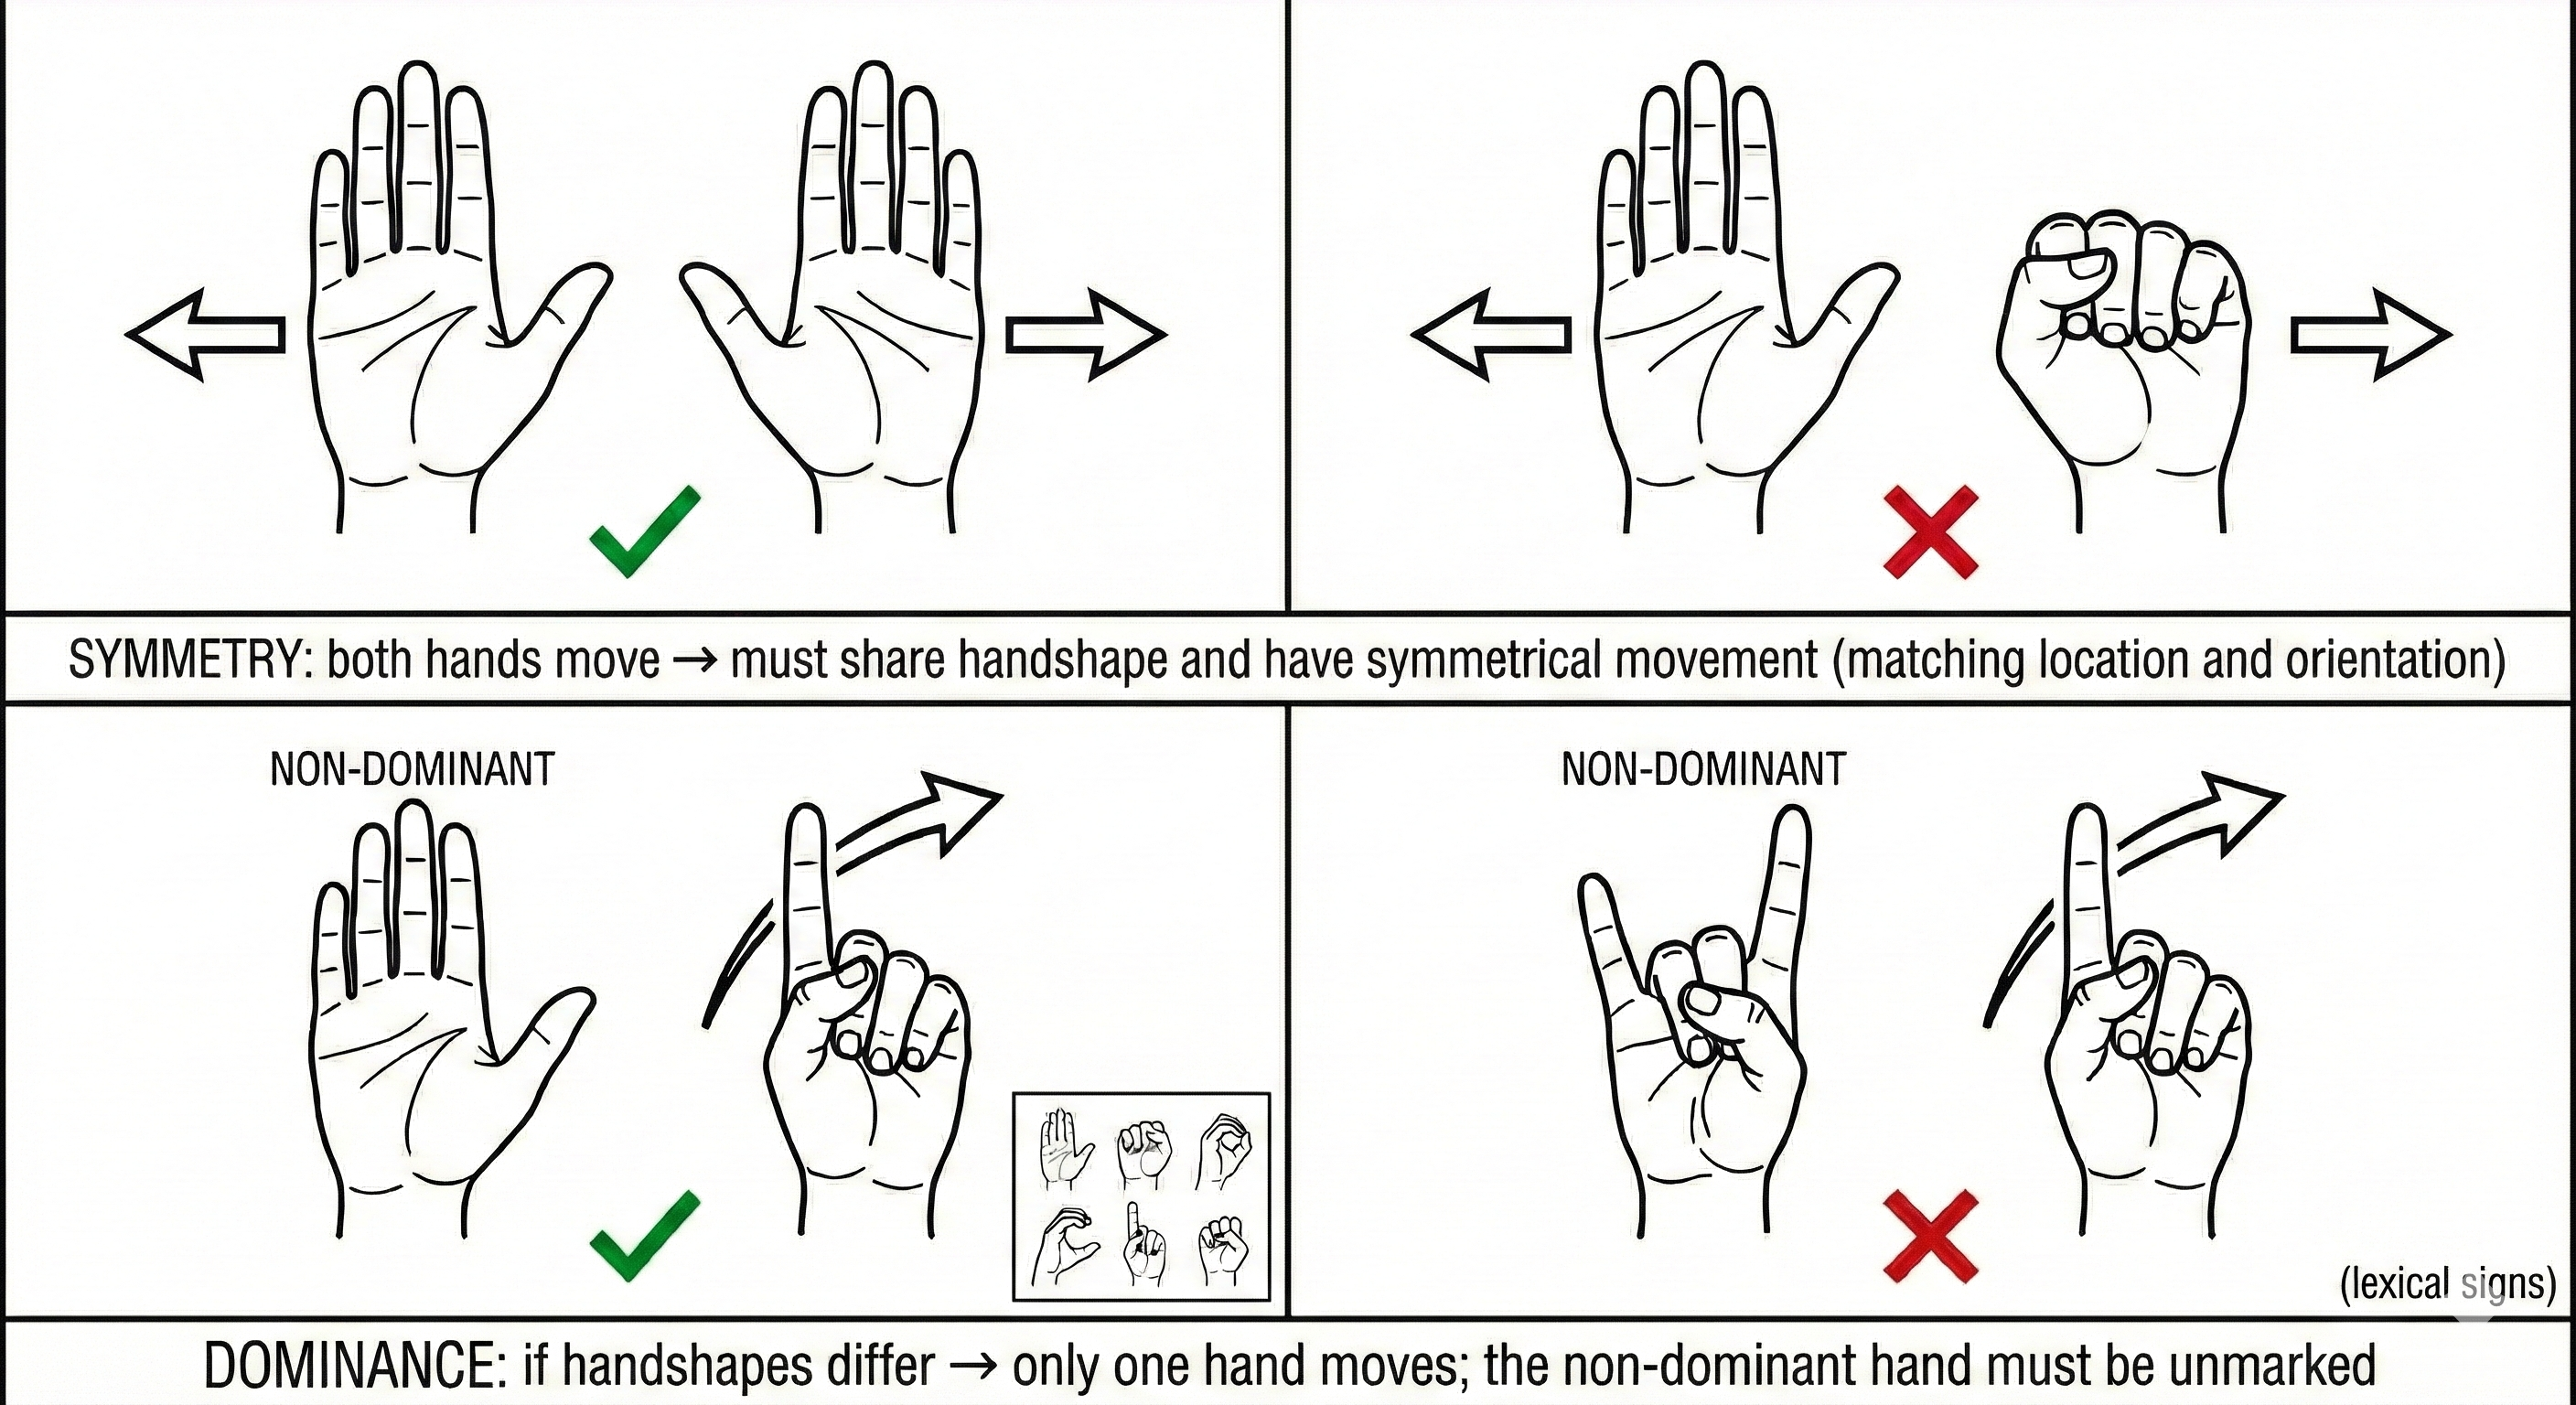
\includegraphics[width=0.85\textwidth]{figures/4.hands.png}
\caption{Phonological constraints in sign languages. Top: the symmetry condition requires that if both hands move, they share handshape and mirror each other's movement. Bottom: the dominance condition requires that if handshapes differ, only one hand moves, and the non-dominant hand uses an unmarked handshape. These constraints emerge independently across unrelated sign languages.}
\label{fig:sign-constraints}
\end{figure}

Nicaraguan Sign Language (ISN) offers near-experimental evidence. ISN emerged in the late 1970s when deaf children were brought together in Managuan schools; no prior sign language was available as a model. Within two generations, ISN developed combinatorial phonology~-- discreteness, duality of patterning, minimal pairs~-- from holistic gestures \citep{senghas2004,senghas2005}. The mechanisms were visible in real time: children segmented continuous gestures into discrete components, regularised variation, imposed categorical structure. Phonological organisation wasn't inherited; it was constructed by the same pressures that maintain it elsewhere.

This suggests the mechanisms maintaining phonological categories are more abstract than vocal-tract physics: categorical perception, motor-planning efficiency, perceptual distinctiveness under noise, learnability across generations \citep{emmorey2002}. These mechanisms operate over whatever articulatory-perceptual channel is available. The substrate varies; the clustering persists. This is HPC in action: different physical realisations, analogous mechanisms, convergent structure.


The framework doesn't need all categories to be HPC kinds. Some categories might be thin~-- lacking the stabilising mechanisms to produce robust clustering, like nonce coinages or idiolectal forms that never diffuse. Some might be fat~-- pooling heterogeneous phenomena under a single label, like cross-linguistic umbrellas that obscure distinct mechanisms. Some might be negative~-- mere complements, wastebasket categories defined by what they're not. Part of the work, going forward, is identifying which grammatical categories are which. Chapter~\ref{ch:failure-modes} develops criteria for diagnosis.


\section{How determinacy survives}
\label{sec:4:determinacy}

A worry hangs over the maintenance view: if categories don't have definitions, how can category membership be determinate? Isn't this just nominalism with extra steps~-- the view that categories are fictions, not facts?

The worry rests on a conflation. Determinacy doesn't require definitions; it requires causal grounding. A tiger is determinately a tiger not because it satisfies a checklist but because of its lineage~-- its causal-historical connection to other tigers, the mechanisms of reproduction and development that produced it. The same goes for grammatical categories. A word is determinately a noun not because it satisfies a definition but because the mechanisms that maintain \term{noun} have operated on it: it was acquired as a noun, used as a noun, aligned with other nouns, transmitted as a noun.

This is Millikan's point about proper functions \citep{millikan1984}. An item's category membership is fixed by its history of production and use~-- by what mechanisms brought it into being and what mechanisms maintain it~-- not by what features it currently displays. The features matter because they're typically produced by the mechanisms. But when history and features diverge, history wins. A malformed tiger~-- one lacking stripes, say~-- is still a tiger because of its lineage. A malformed noun~-- one lacking typical nominal features~-- might still be a noun because of how it was acquired and used.

Where does indeterminacy arise? Where the causal pressures are genuinely mixed or transitional. \mention{Fun} is a hard case not because we lack a definition to apply but because the mechanisms have been pulling in different directions: it was acquired as a noun but is being used increasingly like an adjective, with entrenchment patterns that are genuinely intermediate. The indeterminacy is real, but it's localised~-- a fact about this item in this transitional state~-- not a global fuzziness that infects the whole category.

Compare: are the Larus gulls circling the Arctic a single species or many? As you move around the ring—from Britain through Scandinavia to Siberia to Alaska to California—each population interbreeds with its neighbours. But the endpoints don't: herring gulls and lesser black-backed gulls, meeting in Britain, behave as distinct species. The mechanisms that maintain \mention{species}—reproductive isolation, morphological clustering, ecological niche—are strong at the endpoints and weak at the contact points. The indeterminacy is real, but it's localised to the transitions. No one doubts that robins and eagles are distinct species; the ring species are hard cases precisely where the mechanisms are in tension.

The same will be true for grammatical categories. Most nouns are determinately nouns; most verbs are determinately verbs. The core is stable because the mechanisms maintain it robustly. The periphery is where indeterminacy lives~-- and that's not a problem for the framework; it's a prediction.


\section{Recovering Aristotle}
\label{sec:4:aristotle}

Aristotle has had a longer career as a caricature of essentialism than as a guide to how kinds actually persist. But as Chapter~\ref{ch:essentialism} noted, real Aristotle was subtler. His essences weren't arbitrary definitions; they were supposed to be explanatory. The form of a thing explained its behaviour; the essence was what made the thing the kind of thing it was.

HPC recovers this insight. The homeostatic mechanisms are, in a sense, the essence~-- causally understood. What makes a tiger a tiger is the network of properties maintained by reproduction, development, and selection. What makes a noun a noun is the network of properties maintained by acquisition, entrenchment, alignment, and transmission. The mechanism-cluster \emph{is} the essence, relocated from the definitional to the causal register.

This is why HPC is sometimes called neo-Aristotelian \citep{boyd1999,wilson1999}. It recovers the structure Aristotle wanted~-- real natural kinds with genuine explanatory power~-- without the metaphysical baggage that made classical essentialism untenable. The kinds are real because they support induction. The induction works because the mechanisms maintain the clustering. The clustering is stable because the mechanisms are ongoing. It's a circle, but a virtuous one: mechanisms maintain clusters, and clusters sustain the mechanisms that maintain them.

The recovery isn't complete. Aristotle wanted essences to be intrinsic~-- properties a thing has independently of its relations to other things. HPC kinds are essentially relational: a tiger is a tiger because of its relations to other tigers (lineage), its relations to its environment (selection), its relations to developmental pathways (constraint). Grammatical categories are even more relational: a noun is a noun because of its relations to other nouns (analogy), its relations to speakers (acquisition, entrenchment), its relations to discourse (function). The essentialism being recovered is relational essentialism, not intrinsic essentialism.

That's a feature, not a bug~-- if the phrase itself is a bit prefab, that's fitting, because it trades on the same kind of relational uptake I'm describing. Grammatical categories are inherently relational~-- defined by distribution, opposition, system role. An account that makes them intrinsic would be false to what they are. HPC captures their relational nature while preserving their reality. The categories are real \emph{because} they're relational~-- maintained by relations that keep properties clustered.

A related objection runs deeper. Some philosophers have argued that species are not kinds at all but historical individuals~-- entities with spatiotemporal boundaries rather than classes with members \citep{ghiselin1974,hull1978}. On this view, \mention{tiger} names something more like a scattered object extended through space and time than a category with instances. The distinction matters for some purposes. But individuals, too, are maintained: what makes this tiger \emph{this tiger} over time is not an essence but a cluster of properties held in place by metabolic, developmental, and ecological mechanisms. The HPC question~-- what mechanisms maintain the clustering?~-- applies to individuals as well as to kinds. The species-as-individuals move doesn't escape the maintenance framework; it relocates within it.


\section{The question that remains}
\label{sec:4:remaining-question}

Categories are real because they're maintained. The slogan is clear; the framework is in place. But a puzzle remains.

The framework says categories are property clusters. But the properties underlying grammatical categories~-- frequency, distribution, morphological behaviour, semantic features~-- vary continuously. Frequency is a real number; distribution is a vector; morphological behaviour admits degrees. If the substrates are continuous, how do discrete categories emerge? Why isn't grammar one big blur?

This is the \term{discreteness problem}, and it's not solved by saying \enquote{mechanisms maintain clusters.} Mechanisms can maintain continuous variation just as easily as discrete clumps~-- think of a bell curve, continuously maintained by random variation around a mean. What we need is an account of how mechanisms operating on continuous substrates produce categorical outcomes. Not gradient shading but discrete basins. Not fuzzy boundaries but sharp edges~-- even if the sharpness is achieved rather than given.

Chapter~\ref{ch:discrete-from-continuous} takes up this problem. If the next chapter sometimes looks like bringing a particle accelerator to a sand heap, that is not entirely accidental. The answer will involve scale-dependent tolerance, hyperreal formalisations, and a picture of category boundaries that are sharp but located at inaccessible distances. That may sound like an extravagant toolkit for a familiar-looking question, but each piece earns its keep once we insist on explaining both stability and fuzziness in the same model. Dynamic discreteness, I'll call it~-- discreteness that emerges from the interaction of structure and mechanism.

But the foundation is now in place. Categories are HPC kinds. They're real because they're maintained. What remains is understanding the geometry of the basins they occupy~-- and for that, we turn to how discrete structure emerges from continuous substrates.

